%
% beschleunigung.tex
%
% (c) 2020 Prof Dr Andreas Müller, Hochschule Rapperswil
%
\section{Konvergenzgeschwindigkeit
\label{buch:section:geschwindigkeit}}
\rhead{Konvergenzgeschwindigkeit}
\index{Konvergenzgeschwindigkeit}%
Sind die Fehler einer iterativen numerischen Berechnungsmethoden
bekannt, kann die Gesetzmässigkeit der Fehler ausgenutzt werden,
sie weitgehend zu eliminieren, und so die Konvergenz des Verfahrens
zu beschleunigen.
\index{Fehler eliminieren}%
\index{Fehlergesetz}%
In diesem Abschnitt wollen wir das Prinzip veranschaulichen, es
soll später im Abschnitt~\ref{buch:section:romberg}
bei der Berechnung von Integralen systematisch angewendet werden.

%
% Lineare und quadratische Konvergenz
%
\subsection{Lineare und quadratische Konvergenz
\label{buch:subsection:linearekonvergenz}}
Wir betrachten zwei Beispiele von Iterationsfolgen genauer, die
deutlich unterschiedlich schnell konvergieren.
Ziel ist, diesen Unterschied zu quantifizieren und ein Kriterium
zu finden, welches schnelle Konvergenz von Iterationsfolgen garantiert.

\subsubsection{Lineare Konvergenz}
\index{lineare!Konvergenz}%
\index{Konvergenz!linear}%
Am Beispiel der Iterationsfolge der Funktion $f(x)=\sqrt{x+2}$
von Seite~\pageref{section:beispiel:sqrtiteration}
wurde berechnet, wie sich der Fehler von einer Iteration zur nächsten
entwickelt.
Dabei wurde gefunden, dass der Fehler $\delta_n$ in der $n$-ten Iteration
zu $\delta_{n+1}\approx f'(x^*)\cdot\delta_n$ in der $(n+1)$-ten Iteration
wird.
Sind in der $n$-ten Iteration $k$ Nachkommabits korrekt, ist der Fehler
also von der Grössenordnung $2^{-k}$, wird der Fehler in der $(n+1)$-ten
Iteration von der Grössenordnung $f'(x^*) \cdot 2^{-k}= 2^{-k+\log_2f'(x^*)}$
sein.
In jeder Iteration werden also $\log_2f'(x^*)$ Binärstellen Genauigkeit
gewonnen.

Man sagt, eine Folge ist {\em linear konvergent}, wenn die Anzahl
korrekter Stellen in jeder Iteration um die gleiche Anzahl zunimmt.
\index{konvergent!linear}%
\index{linear konvergent}%
Die Anzahl korrekter Stellen wächst in diesem Fall linear mit der
Anzahl Iterationen.

Für eine konvergente Iterationsfolge einer Funktion $f$ liegt also
normalerweise lineare Konvergenz vor, es werden $\log_2 f'(x^*)$
Binärstellen oder $\log_{10}f'(x^3)$ Dezimalstellen Genauigkeit in
jeder Iteration gewonnen.
Falls die Ableitung $f'(x^*)$ verschwindet liegt offenbar ein
Spezialfall vor, er wird im übernächsten Abschnitt genauer untersucht.

\subsubsection{Quadratische Konvergenz}
\index{quadratische!Konvergenz}%
\index{Konvergenz!quadratisch}%
Ist $x=\sqrt{a}$, dann muss $x = a/x$ gelten, also auch
\[
x = \frac12\biggl(x+\frac{a}x\biggr) = f_a(x).
\]
Mit der Funktion $f_a(x)$ kann man jetzt ein Iterationsfolge konstruieren,
die gegen den Fixpunkt 
\[
x^*=f_a(x^*)
\quad\Rightarrow\quad
x^*=\frac12\biggl(x^*+\frac{a}x^*\biggr)
\quad\Rightarrow\quad
x^{*2}-a=0
\quad\Rightarrow\quad
x^*=\sqrt{a}
\]
von $f_a(x)$ konvergiert.
Wir untersuchen die Konvergenzgeschwindigkeit, indem wir $f_a(x)$
mit Hilfe der Taylor-Reihe approximieren:
\index{Taylor-Reihe}%
\[
f_a(x^*+\delta)
\approx
f_a(x^*) + f_a'(x^*)\cdot\delta + \frac12f''_a(x^*)\cdot\delta^2
\]
Die Ableitungen von $f_a$ sind
\begin{align*}
f'_a(x)
&=
\frac12 -\frac{a}{2x^2}
&&\Rightarrow&
f'_a(x^*)&=0
\\
f''_a(x^*)
&=
\frac{a}{x^3}
&&\Rightarrow&
f''_a(x^*)&=\frac{1}{\!\sqrt{a}}
\end{align*}
Mit $x=x^* =\sqrt{a}$ folgt für den Fehler
\[
f_a(x^*+\delta)
\approx
x^* + \underbrace{\biggl(\frac12-\frac{a}{2x^{*2}}\biggr)}_{\displaystyle=0}\delta
+
\frac{a}{2x^{*3}}\delta^2
=
x^* + \frac{1}{2\sqrt{a}}\delta^2.
\]
Der Fehler wird also im Wesentlichen quadriert.
Sind $k$ Nachkommabits korrekt, liegt ein Fehler von der Grössenordnung
$2^{-k}$ vor. 
Daraus wird in der nächsten Iteration ein Fehler von der Grössenordnung
$2^{-2k}$.
Die Anzahl korrekter Nachkommabits ist $2k$, sie hat sich also
verdoppelt.

Man sagt, eine Folge konvergiert {\em quadratisch} gegen $x^*$,
wenn der Fehler $x_n-x^*$ für $n\to n+1$ quadriert wird, die Anzahl
korrekter Stellen also verdoppelt wird.
\index{konvergent!quadratisch}%
\index{quadratisch konvergent}%
Konvergiert eine Folge quadratisch, werden $N$ korrekte Stellen
innert $\log_2N$ Iterationen erreicht.
Quadratische Konvergenz ist also im Vergleich zu linearer Konvergenz
exponentiell schneller und wird daher in Anwendungen angestrebt.
\index{exponentiell schneller}%

\subsubsection{Konvergenzgeschwindigkeit von Iterationsfolgen}
%
% graphisch2.tex
%
% (c) 2020 Prof Dr Andreas Müller, Hochschule Rapperswil
%
\begin{figure}
\centering
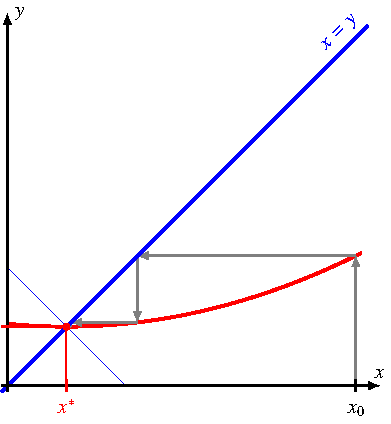
\includegraphics{chapters/10-arithmetik/figures/quadratisch.pdf}
\caption{Die Fixpunktiteration $x_{n+1}=f(x_n)$ konvergiert quadratisch
gegen den Fixpunkt $x^*$
für $f'(x^*)=0$.
\label{buch:figure:fixpunkt:quadratisch}}
\end{figure}

Früher wurde gezeigt, dass die Iterationsfolge $x_{n+1}=f(x_n)$ einer
Funktion $f$ für genügend Nahe bei einem Fixpunkt $x^*$ liegende
Startwerte $x_0$ gegen $x^*$ konvergiert, wenn $|f'(x^*)| < 1$.
Wir sind jetzt auch in der Lage, die Konvergenzgeschwindigkeit
zu quantifizieren.
Dazu entwickeln wird $f(x)$ um $x^*$ bis zur zweiten Ordnung und
erhalten für den Fehler
\begin{equation}
f(x^*+\delta)
\approx
f(x^*) + f'(x^*) \cdot \delta + \frac12f''(x^*)\cdot \delta^2
\label{buch:equation:iterkonv}
\end{equation}
Sofern $f'(x^*)\ne 0$ ist, ist der zweite Term dominant, der Fehler
wird in jeder Iteration mit $f'(x^*)$ multipliziert, es werden in
jeder Iteration $\log_2 f'(x^*)$ Genauigkeit gewonnen.
Es liegt also {\em lineare Konvergenz} vor.
\index{lineare!Konvergenz}%
\index{Konvergenz!linear}%
\index{Iterationsfolge!lineare Konvergenz}%

Verschwindet die Ableitung $f'(x^*)=0$, dann fällt der zweite Term
auf der rechten Seite von~\eqref{buch:equation:iterkonv} weg, der
Fehler ist im wesentlich quadratisch kleiner, es liegt {\em quadratische
Konvergenz} vor.
\index{quadratische!Konvergenz}%
\index{Konvergenz!quadratisch}%
\index{Iterationsfolge!quadratische Konvergenz}%
Diese Situation ist in Abbildung~\ref{buch:figure:fixpunkt:quadratisch}
Wenden wir das Kriterium auf das Beispiel 
\[
f(x) = \frac12\biggl( x + \frac{a}{x}\biggr)
\qquad\text{mit der Ableitung}\qquad
f'(x) = \frac12\biggl( 1 -\frac{a}{x^2}\biggr)
\]
an, finden wir für $f'(x^*)=f'(\sqrt{a}) = 0$.
Die Iterationsfolge muss also quadratisch konvergieren, wie wir
im vorangegangenen Abschnitt auch direkt nachgerechnet haben.

%
% Konvergenzbeschleunigung
%
\subsection{Konvergenzbeschleunigung
\label{buch:subsection:konvergenzbeschleunigung}}
\index{Konvergenzbeschleunigung}%
Die genaue Kenntnis des Fehlers kann auch ermöglichen, einen Teil
des Fehlers zu eliminieren.
Wir illustrieren dieses Prinzip wieder am Beipsiel der Iterationsfolge
\[
x_0,\; x_1=f(x_0),\; x_2=f(x_1),\;x_3=f(x_2),\dots
\]
mit der Funktion $f(x)=\sqrt{x+a}$.
Die Folge konvergiert gegen den Fixpunkt $x^* = f(x^*)$, der
sich durch Quadrieren und Lösen der quadratische
Gleichung
\begin{align*}
x^{*2} &= x^*+a\\
x^{*2} - x^*-a&=0\\
\Rightarrow\qquad
x^* &= \frac12 +\sqrt{\frac14+a}
\end{align*}
finden lässt.
Die negative Wurzel kommt nicht in Frage, weil dies auf eine negative Zahl
führen würde, die nicht Fixpunkt der Wurzelfunktion sein kann, die nur
positive Werte hat.

Wie im früheren Beispiel mit $a=2$ können wir das Verhalten des Fehlers
$\delta_n = x_n-x^*$
mit Hilfe der linearen Approximation
\index{Approximation}%
\[
x_n = x^* + \delta_n
\qquad\Rightarrow\qquad
x_{n+1} = f(x_n) = f(x^* + \delta_n) = f(x^*) + f'(x^*)\cdot \delta_n
=
x^* + \underbrace{f'(x^*)\cdot \delta_n}_{\displaystyle\approx\delta_{n+1}}
\]
ermitteln.
Der Fehler wird also in jeder Iteration um den Faktor
\[
f'(x^*) = \frac1{2\sqrt{x^*+a}}=\frac1{2x^*}
\]
kleiner.
Wir wissen somit, dass der Fehler in jeder Iteration um den
{\em gleichen} Faktor
kleiner wird, aber da wir $x^*$ noch nicht kennen, kennen wir den Wert $q$
des Faktors noch nicht.

Drei aufeinanderfolgende Folgenglieder sind
\begin{align}
x_{n-1}           &= x^* + \phantom{q^2}\delta
\notag
\\
x_{n\phantom{-0}} &= x^* + q^{\phantom{2}}\delta
\label{buch:equation:sqrtbeschl1}
\\
x_{n+1}           &= x^* + q^2\delta
\label{buch:equation:sqrtbeschl2}
\end{align}
Darin sind alle drei Grössen auf der rechten Seite unbekannt.
Die Differenzen aufeinanderfolgender Folgenglieder sind
\begin{align*}
x_{n\phantom{\mathstrut-0}} - x_{n-1} &= \delta(q-1)                  \\
x_{n+1}-x_{n\phantom{\mathstrut -0}}  &= \delta(q^2-q) =\delta q(q-1).
\end{align*}
Der Differenzenquotient
\index{Differenzenquotient}%
\[
\frac{
x_{n+1}-x_{n\phantom{\mathstrut -0}}
}{
x_{n\phantom{\mathstrut-0}} - x_{n-1}
}
=q
\]
kann verwendet werden, eine bessere Approximation zu bestimmen.
Dazu multipliziert man~\eqref{buch:equation:sqrtbeschl1} mit $q$
und subtrahiert das Resultate von~\eqref{buch:equation:sqrtbeschl2}.
Man erhalt
\[
x_{n+1}- qx_n = (1-q) x^*
\qquad
\Rightarrow
\qquad
x^* = \frac{x_{n+1}-qx_n}{1-q}.
\]
Damit können wir eine neue Iteration definieren:
\begin{enumerate}
\item Berechne aus $x_0$ die Werte $x_1=f(x_0)$ und $x_2=f(x_1)$.
\item Berechne
\[
q = \frac{x_2-x_1}{x_1-x_0}
\qquad\text{und}\qquad
x^* = \frac{x_{2}-qx_1}{1-q}.
\]
\item Setze $x_0 = x^*$ und beginne bei 1.
\end{enumerate}

\begin{table}
\centering
\renewcommand\arraystretch{1.15}
\begin{tabular}{|>{$}r<{$}| >{$}r<{$} | >{$}r<{$} | >{$}r<{$} |}
\hline
k&\text{Fixpunkt}&\text{Fehler}&q\\
\hline
1 & \underline{2.0}39426062845019 & 0.039426062845019 & 0.306 \\
2 & \underline{2.00000}8018463113 & 0.000008018463113 & 0.249 \\
3 & \underline{2.000000000000}335 & 0.000000000000335 & 0.249 \\
4 & \underline{2.000000000000000} & 0.000000000000000 & 0.249 \\
\hline
\end{tabular}
\caption{Resultate des beschleunigten Verfahrens zur Bestimmung eines
Fixpunktes der Iterationsfolge der Funktino $f(x)=\sqrt{x+a}$ mit $a=2$.
\index{Fixpunkt}%
\label{buch:table:sqrtbeschl}}
\end{table}

Das neue Verfahren zur Berechnung des Fixpunktes konvergiert jetzt
viel schneller, wie die Resulate in Tabelle~\ref{buch:table:sqrtbeschl}
zeigen.
\index{Fixpunkt}%
Die Konvergenz ist sehr rasch, es scheint als ob sich in jeder
Iteration die Anzahl der korrekten Stellen verdoppelt, dass also
quadratische Konvergenz vorliegt.
Dies lässt sich auch mit Hilfe einer analytischen Rechnung
bestätigen.
Dazu approximiert man $f(x^*+\delta)$ bis zu Termen zweiter Ordnung,
also als
\[
f(x^*+\delta)
=
f(x^*) + f'(x^*)\cdot \delta + \frac12f''(x^*)\cdot \delta^2+ \dots,
=
x^* + q\delta + b\delta^2
\]
verwendet dies für die Analyse des neuen Iterationsverfahrens.
Wir schreiben also
\begin{align}
x_0
&=
x^* + \delta
\label{buch:equation:sqrtbeschllin}
\\
x_1
&=
x^* + q\delta + b\delta^2
\notag
\\
x_2
&=
x^* + q(q\delta+b\delta^2) + b(q\delta+b\delta^2)^2
     = x^* + q^2 \delta + qb\delta^2 + bq^2\delta^2
	+ 2qb^2\delta^3 + b^3\delta^4
\notag
\\
&=
x^* + q^2\delta + qb(1+q)\delta^2
\notag
\end{align}
und wenden den neuen Algorithmus darauf an.
Der Quotient ist
\begin{align*}
\frac{x_2-x_1}{x_1-x_0}
&=
\frac{x^* + q^2\delta + qb(1+q)\delta^2 - 
(x^* + q\delta + b\delta^2)}{
x^* + q\delta + b\delta^2
-
(x^* + \delta)
}
=
\frac{
q(q-1)\delta + b(q^2+q -1) \delta^2
}{
(q-1)\delta + b\delta^2
}
\\
&\approx
\frac{q(q-1)\delta}{(q-1)\delta}
=
q.
\end{align*}
In der zweiten Zeile gehen wir davon aus, dass $\delta^2 \ll \delta$ und
dass daher die Terme mit $\delta^2$ im Bruch vernachlässigt werden dürfen.
Nache dem zweiten Schritt des Algorithmus ist der neue Näherungswert
von $x^*$ gegeben durch
\begin{align}
\frac{x_2-qx_1}{1-q}
&=
\frac{
x^* + q^2\delta + qb(1+q)\delta^2
-q(
x^* + q\delta + b\delta^2
)
}{
1-q
}
=
\frac{ (1-q)x^* + qb(1+q)\delta^2 - qb\delta^2 }{1-q}
\label{buch:equation:sqrtnext}
\\
&=
x^* + \frac{q^2b}{1-q}\delta^2.
\label{buch:equation:sqrtbeschlquadrat}
\end{align}
Der ursprüngliche Fehler $\delta$ in 
\eqref{buch:equation:sqrtbeschllin}
wurde
durch die Iteration
nach
\eqref{buch:equation:sqrtbeschlquadrat}
im wesentlichen quadriert worden.
Damit ist die quadratische Konvergenz bestätigt.

Ein fairer Vergleich der Konvergenzgeschwindigkeit der usprünglichen
Iterationsfolge mit dem neuen Algorithmus sollte die Anzahl der
Auswertungen der Funktion $f$ mit zählen. 
\index{Auswertungen}%
\index{Funktionsauswertungen}%
In der ursprünglichen Iterationsfolge wird in jeder Iteration die 
Funktion einmal ausgewertet, der neue Algorithmus braucht zwei
Funktionsauswertungen pro Iteration.
In der ursprünglichen Iterationsfolge wurden 52 bit Genauigkeit nach
26 Schritten und damit nach 26 Funktionsauswertungen erreicht.
Die neue Folge erreicht Konvergenz in 4 Iterationen und damit 8
Funktionsauswertungen.
Auch unter Berücksichtigung der Anzahl Funktionsauswertungen ist
das neue Verfahren bedeutend weniger aufwendig.

Trotz dieses spektakulären Erfolgs der Konvergenzbeschleunigung weist das
Verfahren für praktische Rechnungen einige entscheidende Mängel auf.
Da die Folge gegen $x^*$ konvergiert, werden 
die Werte $x_0$, $x_1$ und $x_2$ fast gleich gross sein, so dass es
zu Auslöschung und damit zu Werten sehr geringer Genauigkeit für $q$
kommen kann.
\index{Auslöschung}%
Ein solcher Fehler in $q$ schlägt sich wegen
\eqref{buch:equation:sqrtnext}
sofort auch im nächsten Approximationswert für $x^*$ nieder.

Im Abschnitt~\ref{buch:section:romberg} wird am Beispiel des
Romberg-Integrationsverfahrens gezeigt, wie die Konvergenz der
Integralberechnung mit der Trapezregel beschleunigt werden kann.
\index{Romberg-Integration}%
\index{Trapezregel}%




